% !TEX root = 00_arbeit.tex

%---------------------------------------------------------------------------------
%% Theorie

\section{Künstliche Neuronale Netze}

In diesem Kapitel werden zunächst biologische und künstliche neuronale Netze verglichen. Gefolgt von einer Motivation über die Verwendung künstlicher neuronaler Netze (zukünftig als NN bezeichnet) und der Einordnung der NN in die aktuelle Forschungslanschaft. Als nächstes werden die Charakterisierungskriterien für NN vorgestellt und ein Überblick über mögliche Anwendungsgebiete für NN gegeben. Anschließend wird ein Überblick über die Funktionsweise gängiger Modelle gegeben und die Netzwerkmodelle gegenübergestellt.

\subsection{Einleitung in Neuronale Netze}
%\farbig{[Erklärung der neuronalen Netze... vielfältige Anwendungsgebiete... Hier erforderlich Netze zur Zeitreihenvorhersage]}
%\setlength{\intextsep}{0pt}%

%\begin{wrapfigure}{r}{0.5\textwidth}
%    \centering
%        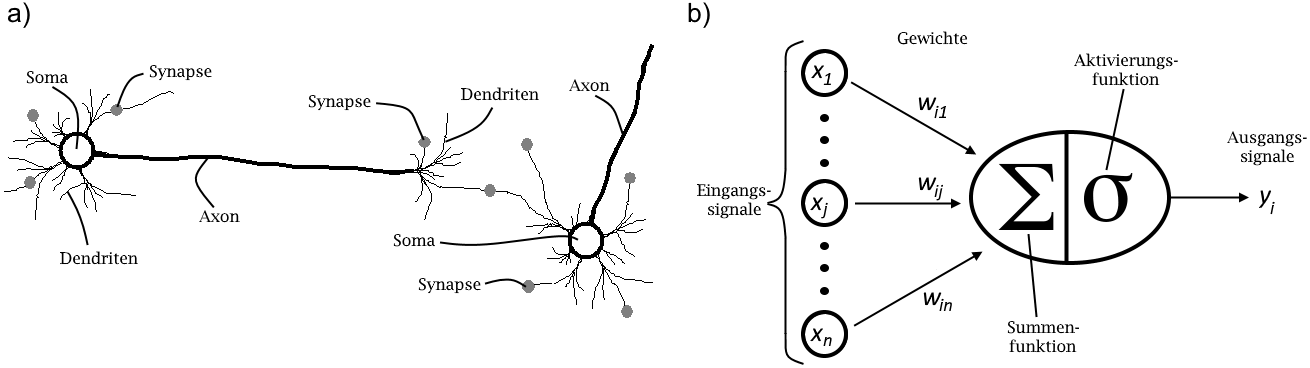
\includegraphics[width=0.5\textwidth]{Bilder/BNN_ANN.png}
%    \caption{Gegenüberstellung eines Ausschnittes aus einem biologischen neuronalen Netz a)\protect\footnotemark{} und einem künstlichen neuronalen Netz b).}
%    \label{fig:BNN_ANN}
%\end{wrapfigure}


%\citet[\pno~2~ff.]{sen_an}

Ein künstliches neuronales Netz (engl. artificial neural networks)~(NN) ist ein mathematisches Konstrukt. Es bildet ein informationsverarbeitendes System welches aus einer Vielzahl einfacher Einheiten den sogenannten Neuronen besteht. Entstanden ist es Anfang der 40er Jahre des letzten Jahrhunderts\citef[A1.1:1]{Fiesler96} aus der Untersuchung von biologischen Abläufen im Nervensystem von Wirbeltieren, wo Sinneseindrücke des Körpers aufgenommen und mit Hilfe diverser neuronaler Netze verarbeitet werden.

\begin{figure}[!htb]
    \centering
        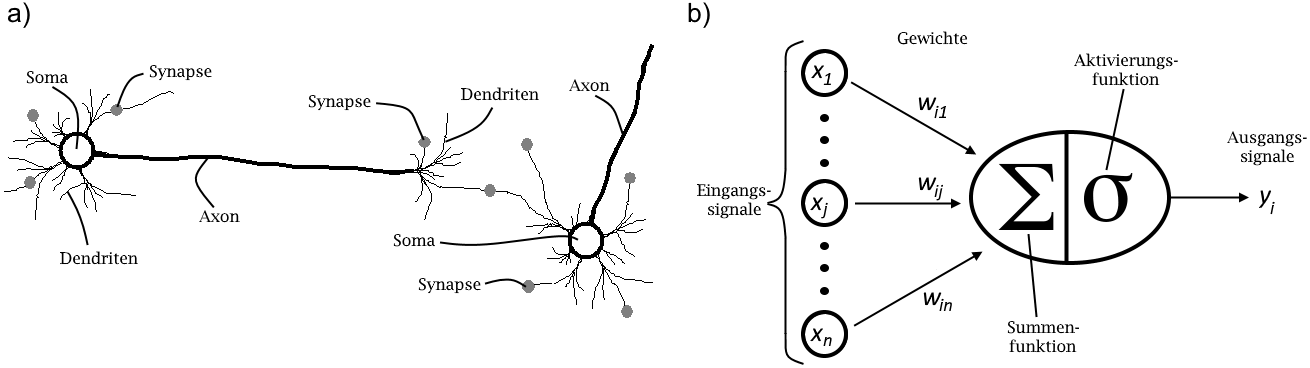
\includegraphics[width=1\textwidth]{Bilder/BNN_ANN.png}
    \caption{Gegenüberstellung eines Ausschnittes aus einem biologischen neuronalen Netz a)\protect\footnotemark{} und einem künstlichen neuronalen Netz b).}
    \label{fig:BNN_ANN}
\end{figure}

\addtocounter{footnote}{-1}     %  -1 mal die Gesamtanzahl an Fußnoten in der wrapfigure
\addtocounter{Hfootnote}{-1}    % -1 times total number of footnote(mark)s in the wrapfigure
\wrapfigfoot\footnotetext{\autoref{fig:BNN_ANN} a) wurde aus\citet[2]{sen_an} übersetzt und angepasst.}

\autoref{fig:BNN_ANN} zeigt eine Gegenüberstellung eines künstlichen und biologischen Neurons. Dabei können die Dendriten eines biologischen Neurons als Informationseingang, das Axon als Informationsausgang, die Synapsen als Gewichte und die Soma als Summen- und Aktivierungsfunktion des künstlichen Neurons angesehen werden. 

\todo{Als Grundmodell für das ktinstliche Neuron diente das neurophysiologische Vorbild, das auf McCulloch und Pitts (aaO.) zurtickzufUhren ist. Diese betrachteten ein Neuron als eine Art Addierer der ankommenden Impulse, die durch die Dendriten (Eingangs-kanale) aufgenommen werden. Die Aktivitaten, mit einer bestimmten Gewichtung, werden im Soma (Korper des Neurons mit Zellkem) summiert und, sofem die Summe einen bestimmten Schwellwertüberschreitet, wird die Information durch das Axon (Ausgangskanal) weitergeleitet. Der Kontakt zu den anderen Neuronen findet tiber Synapsen (elektrochemische Kontakte) statt. Diese konnen die kontaktierten Neuronen hemmen bzw. erregen (vgl. Stanley und Bak, 1991; Brause, 1991; Schoneburg u.a., 1990; Ritter u.a., 1991)  $doi:https://doi.org/10.1007/978-3-322-83450-8\_2 - S.17$}


Das zurzeit prominenteste künstliche Neuron (die kleinste Einheit im Netzwerk), dargestellt in \hbox{\autoref{fig:BNN_ANN} b)}, wird nach \citet{perceptron_ros58} als Perceptron bezeichnet. Es verarbeitet die Eingangssignale über die Propagierungsfunktion. In \autoref{fig:BNN_ANN} b) ist es die Summenfunktion. So summiert es zunächst die gewichteten Eingangsinformationen mit $\varphi (x)=\sum_{i=1}^{n}x_{i}\omega_{i}$, anschließend wird die gewichtete Summe~$\varphi(x)$ über die Aktivierungsfunktion~$\sigma(x)$ als Ausgang~$y$ an das nächste Neuron übergeben.
%
%
%\setlength{\intextsep}{0pt}%
%\setlength{\columnsep}{10pt}%
%\begin{wraptable}{l}{6.4cm}
%    \caption {Analogie zwischen biologischen und künstlichen Neuronen.}
%   \begin{tabular}{>{\centering\arraybackslash}m{2.2cm}>{\centering\arraybackslash}m{3.4cm}}
%    \hline
%    Biologisches\newline Neuron & Künstliches\newline Neuron            \\ \hline \hline
%    Soma                & Summen- und\newline Aktivierungsfunktion      \\ 
%    Dendrit             & Eingang                                       \\ 
%    Axon                & Ausgang                                       \\ 
%    Synapse             & Gewicht                                       \\ \hline
%    \end{tabular}
%    \label{tab:BNN_ANN}
%\end{wraptable}
%

Klassische Aktivierungsfunktionen sind in \autoref{fig:funktion} dargestellt. Wobei die \hbox{Heaviside-,} die lineare Schwellwertfunktion und der Tangens Hyperbolicus bipolar dargestellt sind (Wertebereich [-1,1]) aber auch unipolar (Wertebereich [0,1]) darstellbar sind. Die Fermifunktion weist zwar nur einen Wertebereich von [0,1] auf aber durch den Temperaturfaktor kann sie an die Heavisidefunktion angenährt werden und hat den Vorteil der Differenzierbarkeit.\footnote{Vgl. \citet[5]{neuralnet_intro} und \citet[39 f]{dkriesel07}.}

\begin{figure}[!htb]
    \centering
        %---------------------------------------------------------------
        %% Heaviside
        \begin{tikzpicture}[scale=.7,font=\scriptsize,thick,>=stealth']
            \coordinate (O) at (0,0);
            % horizontal axis
            \draw[->] (-0.3,0) -- (4,0) coordinate[label = {right:$x$}] (xmax);
            % vertical axis
            \draw[->] (0,0) -- (0,2) coordinate[label = {above:$f(x)$}] (ymax);
  
            \node[align=center] at (2,3) {Heaviside-\\funktion};
  
            \draw (2,2) -- (4,2);
            \draw (2,-2) -- (0,-2);
            \draw[dashed] (2,2) -- (2,-2);
        \end{tikzpicture}
        %---------------------------------------------------------------
        %% lineare Schwellwertfunktion
        \begin{tikzpicture}[scale=.7,font=\scriptsize,thick,>=stealth']
            \coordinate (O) at (0,0);
            % horizontal axis
            \draw[->] (-0.3,0) -- (4,0) coordinate[label = {right:$x$}] (xmax);
            % vertical axis
            \draw[->] (0,0) -- (0,2) coordinate[label = {above:$f(x)$}] (ymax);
  
            \node[align=center] at (2,3) {lineare\\Schwellwert-\\funktion};
  
            \draw (3,2) -- (4,2);
            \draw (1,-2) -- (0,-2);
            \draw (1,-2) -- (3,2);
        \end{tikzpicture}
        %---------------------------------------------------------------
        %% Fermifunktion
        \begin{tikzpicture}[scale=.7,font=\scriptsize,thick,>=stealth']
            \draw[white] (1,-2) -- (3,2);
            \draw[scale=.5,domain=-4:4,smooth,variable=\x,lightgray]      plot ({\x+4},{4*(1/(exp(-\x/.2)+1))});
            \draw[scale=.5,domain=-4:4,smooth,variable=\x,lightgray]      plot ({\x+4},{4*(1/(exp(-\x/.5)+1))});
            \draw[scale=.5,domain=-4:4,smooth,variable=\x,black]          plot ({\x+4},{4*(1/(exp(-\x/.8)+1))});
            % horizontal axis
            \draw[->] (-0.3,0) -- (4,0) coordinate[label = {right:$x$}] (xmax);
            % vertical axis
            \draw[->] (0,0) -- (0,2) coordinate[label = {above:$f(x)$}] (ymax);
            \node[align=center] at (2,3) {Fermifunktion};
        \end{tikzpicture}
        %---------------------------------------------------------------
        %% Tangens Hyperbolicus
        \begin{tikzpicture}[scale=.7,font=\scriptsize,thick,>=stealth']
            \coordinate (O) at (0,0);
            % horizontal axis
            \draw[->] (-0.3,0) -- (4,0) coordinate[label = {right:$x$}] (xmax);
            % vertical axis
            \draw[->] (0,0) -- (0,2) coordinate[label = {above:$f(x)$}] (ymax);
            \node[align=center] at (2,3) {Tangens\\Hyperbolicus};
            \draw[scale=0.5,domain=-4:4,smooth,variable=\x,black] plot ({\x+4},{4*tanh(\x)});
        \end{tikzpicture}

    \caption{Typische Funktionen die als Aktivierungsfunktion angewendet werden.}
    \label{fig:funktion}
\end{figure}

Es gibt Problemstellungen die mit klassischen mathematischen Modellen und Algorithmen gar nicht oder nur schwer zu lösen sind. Neuronale Netze unterscheiden sich zu klassischen Algorithmen durch ihre Lernfähigkeit. Ohne explizite Programmierung sind sie in der Lage eine Aufgabe anhand von Trainingsbeispielen zu erlernen. Einige Beispiele wären die Gesichtserkennung oder die Erkennung von menschlicher Sprache.\\

%\newpage

Künstliche neuronale Netze sind augenblicklich eine Disziplin der Computional Intelligence~(CI), welches wiederum einen Teilbereich der Künstlichenintelligenz (artificial intelligence)~(AI) darstellt. Diese fasst verschiedene von der Natur inspirierte Berechnungsmethoden zusammen. Weitere Methoden der CI sind Fuzzy-Systeme~(FS), Evolutionäre Algorithmen~(EA), Schwarmintelligenz~(SI) und Künstliche Immunsysteme~(AIS).\citef[11 ff]{Kroll16} Obwohl sich diese Arbeit wesentlich mit NN beschäftigen wird, wird an dieser Stelle auf weitere CI-Methoden hingewiesen, da in der Literatur hybride CI-Systeme bekannt sind und auch genutzt werden.

\subsection{Charakterisierung und Anwendung künstlicher neuronaler Netze}

Da es nicht das NN gibt sondern viele unterschiedliche Arten, die teilweise spezielle Anwendungsgebiete finden, werden in diesem Unterkapitel Charakterisierungskriterien für NN vorgestellt. Schließlich wird ein Überblick über mögliche Anwendungsgebiete gegeben.\\

Im allgemeinen können NN anhand der folgenden drei Kriterien charakterisiert werden\citef[7 ff]{characterisation_4}:%

\begin{enumerate}
\item%
Nach der Art des verwendeten Neurons.\\
Dazu gibt es in der Literatur vielfältige Beispiele. \citet{Fiesler96} zählen einige Beispiele im Kapitel B1 auf und weisen auf Unterschiede hin. Als Beispiel wird dort das bereits erwähnte Perceptron beschrieben. Dann gehen sie auf das Neuron des Hopfield-Netzwerkes ein, bei dem das Neuron ein Teilchen beschreibt welches sich in einem Magnetfeld ausrichtet. Ein eher exotischer Vertreter der dort nicht erwähnt wird ist das Fuzzy-Neuron von \citet{fuzzy-neuron}, welches nach der Aktivierung mehrere mögliche Zustände einnehmen kann und seine Anwendung in der Mustererkennug findet.

\item%
Nach der Topologie buw. der Verbindungsarchitektur.\\
Sie beschreibt wie Neuronen in einem Netzwerk verbunden sind.
Es werden folgende Architekturen unterschieden:
\begin{itemize}
\item[\textbf{$\bullet$}]%
Autoassoziative: Hierbei fungieren die Eingangs- gleichzeitig als Ausgangsneurone (z.B. das Hopfield-Netzwerk). 

\item[\textbf{$\bullet$}]%
Heteroassoziative: Unterschiedliche Neurone übernehmen die Rolle der Eingangs- bzw. Ausgangsneurone. Hierzu zählen die Multi-layer-Perceptrons (MLP) bei dem mehrere Schichten von mehrzahligen Perceptrons ein Netzwerk Bilden\citef[86 ff]{dkriesel07}. Aber auch das Kohonen Netzwerk auch bekannt als Self Organizing Maps (SOM) bei dem die Neuronen sich selbständig anordnen und der Zustand des Netzes als Ausgabe dient\citef[153 ff]{dkriesel07}.

Zusätzlich wird unterschieden wie die Verbindungen unter den einzelnen Neuronen realisiert sind. Hier wird zwischen zwei Arten unterschieden:

\item[$\circ$]%
Feed-Forward: Diese Netzwerke bestehen meistens aus Schichten und eine Schicht ist nur mit der jeweils nächsten Schicht verbunden.

\item[$\circ$]%
Recurrent (Feed-Back): In der deutschsprachigen Literatur als rückgekoppelte oder rekurrente Netze bezeichnet beeinflussen sich diese Netzwerke selbst. Die Neuronen dieser Netzwerke besitzen eine Verbindung entweder zu sich selbst (direkte Rückkoppelung), zu den Neuronen der vorhergehenden Schicht (indirekte Rückkopplung), zu den Neuronen der gleichen Schicht (laterale Rückkopplung) oder vollständig verbundene Netze (Verbindungen zwischen allen Neuronen ausgenommen der direkten Rückkopplung). Durch die Rückkopplung besitzen diese Netzwerke ein ``Gedächtnis''~da der vorherige Zustand in die Auswertung der aktuellen Eingangsinformation mit einfließt.\citef[42 ff]{dkriesel07} Ein Beispiel für ein vollständig verbundenes Netzwerk ist das Hopfield-Netzwerk.

\end{itemize}

\item%
Nach dem Lernalgorithmus. Dieser ermöglicht es das Netzwerk zu trainieren. Die heutzutage benutzten Algorithmen werden in drei Gruppen unterteilt\footnote{Vgl. \citet[55]{dkriesel07}.\label{kriesel55}}:

\begin{itemize}
\item[\textbf{$\bullet$}]%
Supervised learning (überwachtes Lernen): Die Trainingsbeispiele bestehen aus einer Menge an Eingangsinformationen und den dazugehörigen Ausbangsinformationen. Das Ziel ist es die Differenz zwischen der tatsächlichen Ausgabe des Netzwerks und den vorliegenden Ausgangsinformationen zu minimieren.

\item[\textbf{$\bullet$}]%
Reinforcement learning (bestärkendes Lernen): Plakativ kann diese Lernmethode als Zuckerbrot und Peitsche bezeichnet werden bzw. lernen durch Belohnung und Bestrafung. Hierbei werden die Eingangsinformationen zur Verfügung gestellt und die Ausgabe des Netzwerkes wird anhand einer Belohnungsfunktion bewertet. Wird die Ausgabe als gut/schlecht angesehen so werden die zugehörigen Verbindungen gestärkt/geschwächt\footnote{Vgl. \citet[201]{dkriesel07} und \citet[A2.3:5]{Fiesler96}.}. 

\item[\textbf{$\bullet$}]%
Unsupervised learning (unüberwachtes Lernen): Wird auch als selbstorganisiertes (self organized) Lernen bezeichnet. Die Trainingsbeispiele bestehen hierbei nur aus Eingansinformationen. Das Netzwerk versucht aus den Eingansinformationen selbstständig Ähnlichkeiten zu erkennen.
Unüberwachte Lernmethoden werden noch unterteilt in konkurrierendes (competitive) und nicht konkurrierendes (noncompetitive) Lernverfahren. Der unterschied besteht darin dass bei dem konkurrierenden Verfahren in einem Netzwerk einzelne Gruppen von Neuronen um die Aktivität konkurrieren\citef[B3.3:5]{Fiesler96}.

Zusätzlich unterscheidet man unter allen drei Lernmethoden zwei Lernarten\citef[A2.3:3]{Fiesler96}: 
\item[$\circ$]%
off-line learning: Auch Batch-Trainingsverfahren genannt. Hierbei wird die Netzwerkausgabe nach einer Menge von Eingangsinformationnen ausgewertet und anschließend werden die Gewichte angepasst.

\item[$\circ$]%
on-line learning: Hier werden die Gewichte nach jeder einzelnen Beobachtung der gesamten Eingangsinformationen angepasst. 

\end{itemize}

\end{enumerate}

Vollständigkeitshalber wird erwähnt, dass \citet{characterisation_4} vier Charakterisierungskriterien nennen. Wobei als viertes Kriterium der Informationsgewinnungsalgorithmus (recall algorithm) aufgeführt ist. In dieser Arbeit wird auf dieses Kriterium verzichtet, da weder \citet{characterisation_4} eine Einteilung/Auflistung aufführen noch in anderer Literatur dieses Kriterium eine Erwähnung findet.\\

Es gibt vielfältige Anwendungsgebiete für NN. Angefangen bei Optimierungsproblemen, wo das Ziel es ist optimale Werte für ein gegebenes System zu finden. Über die Datenverarbeiteung, wo Bild- bzw. Sprachinformationen verarbeitet, generiert oder komprimiert werden. Bis zur Klassifikation/Erkennung von Mustern, wo es darum geht aus einer Dantemenge zusammenhängende Muster zu erkennen. Weitere Anwendungen sind die Kontrelle/Regelung von industriellen Anlagen und die wichtigste (bezogen auf diese Arbeit) ist die Funktionsapproximation bzw. Zeitreihenmodellierung, wo die Beziehung aus Eingangsinformationen und dem gewünschtem Ausgang zu finden gilt. Dies sind einige kurz umrissene Anwendungsbeispiele. In der Literatur werden deutlich mehr Bespiele aufgeführt.\footnote{Vgl. \citet[224]{Kroll16}, \citet[15]{comp_int_07} und \citet[F1 ff]{Fiesler96}.}\\

%\farbig{NN sind Black-Box und Analyse ist schwer aber es gibt in der Literatur mögliche Analyseverfahren.}


\subsection{Überblick über gängige Modelle}
Im vorherigen Kapitel wurde die Charakterisierung der NN beleuchtet und einige Netzwerkmodelle mit ihren Anwendungen genannt. In diesem Kapitel soll die Funktionsweise näher erläutert werden.

\subsubsection{Perceptrons (SLP)/(MLP)}
\begin{figure}[!htb]
    \centering
        %---------------------------------------------------------------
        %% SLP
        %-----------------------------------------
        %% linkes Bild
        \begin{tikzpicture}[>=stealth', node distance=\layersep cm, shorten >=1pt]
        \def\layersep{2}            % vertikal distance between the layers
        \def\neuronsep{1.5}         % Horizontal distance between neurons
        \def\dlsize{1.5}            % distance between node and layer lable
        \def\inout{\layersep*.65}   % Size of in- and output-arrow
        \def\siz{.8}                % neuronsize
        \def\y{3}                   % Start of the most upper layer
        \def\ni{5}                  % Amount of input neurons
        \def\no{2}                  % Amount of output neurons
        \tikzstyle{neuron}=[circle,draw=black,minimum size=\siz cm,inner sep=2pt]
        \tikzstyle{annot} = [text width=5em, text centered]
        \tikzset{fontscale/.style = {font={\fontsize{#1pt}{#1pt}\selectfont}}}
        \newcommand{\neurono}[2][]{
            \node[neuron,circle split,inner sep=2pt] (#1) at (#2)
                    {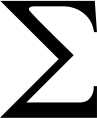
\includegraphics[width=0.225cm]{Bilder/Sigma.png} \nodepart{lower} 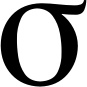
\includegraphics[width=0.225cm]{Bilder/sigma.png}};
        }

        % Draw the left input layer nodes
            \foreach \name / \xn in {1,...,\ni}{
            % This is the same as writing \foreach \name / \y in {1/1,2/2,3/3,4/4}
                \node[neuron,fontscale=15] (Il-\name) at (\xn*\neuronsep-\neuronsep,\y) {$i_{\xn}$};
                \node[above of=Il-\name, node distance=\inout cm] (Inl-\name) {};
                \draw [->,arrows={-Stealth[length=7pt]},densely dotted] (Inl-\name) edge (Il-\name);
            }
        % Draw the output layer node
            \foreach \name / \xn in {1,...,\no}{
                \node[neuron,fontscale=15] (Ol-\xn) at ({(\ni-1)*\neuronsep/2-\neuronsep/2*(\no-1)+(\xn-1)*\neuronsep},\y-\layersep) {$\Omega_{\xn}$};
                \node[node distance=\inout cm, below of=Ol-\xn] (Onl) {};
                \draw [->,arrows={-Stealth[length=7pt]},densely dotted] (Ol-\xn) edge (Onl);
        % Connect every node in the input layer with the output layer
            \foreach \source in {1,...,\ni}
                \draw [->,arrows={-Stealth[length=7pt]}] (Il-\source) edge (Ol-\xn);
                }
        % Annotate the layers
                \node[annot,right of=Il-\ni, node distance=\dlsize cm] (il) {\textbf{Eingabe- schicht}};
                \node[annot,below of=il] {\textbf{Ausgabe- schicht}};
        %-----------------------------------------
        %% rechtes Bild
            \tikzset{
                ident/.pic={
                \draw[semithick] (-\siz/4,-\siz/4) -- (\siz/4,\siz/4);
            }}
        % Draw the right input layer nodes
                \node[xshift=\dlsize cm] (Ir) at (il) {};
            \foreach \name / \xn in {1,...,\ni}{
        % This is the same as writing \foreach \name / \y in {1/1,2/2,3/3,4/4}
                \node[neuron] (Ir-\name) at ($(Ir)+(\xn*\neuronsep-\neuronsep,0)$) {};
                \node[above of=Ir-\name, node distance=\inout cm] (Inr-\name) {};
                \pic at (Ir-\name) {ident};
                \draw [->,arrows={-Stealth[length=7pt]},densely dotted] (Inr-\name) edge (Ir-\name);
            } 
        % Draw the output layer node
            \foreach \name / \xn in {1,...,\no}{
                \neurono[Or-\xn]{$(Ir)+({(\ni-1)*\neuronsep/2-\neuronsep/2*(\no-1)+(\xn-1)*\neuronsep},-\layersep)$}

                \node[node distance=\inout cm, below of=Or-\xn] (Onr) {};
                
                \draw [->,arrows={-Stealth[length=7pt]},densely dotted] (Or-\xn) edge (Onr);
                
        % Connect every node in the input layer with the output layer
            \foreach \source in {1,...,\ni}
                \draw [->,arrows={-Stealth[length=7pt]},every node/.style={fill=white,inner sep=1pt,fontscale=7}] 
                (Ir-\source) edge  (Or-\xn) 
                node at ($(Ir-\source)!.3+.18*(\xn-1)!(Or-\xn)$) {$w_{\source,\xn}$};
            }
\end{tikzpicture}
        %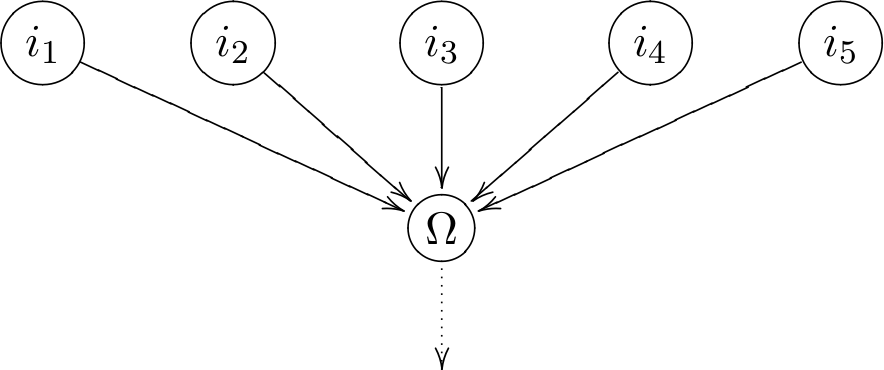
\includegraphics[width=.5\textwidth]{Bilder/MLP/slp.png}
    \caption{SLP mit fünf Eingabeneuronen $i_n$ und einem Ausgabeneuron $\Omega$.}
    \label{fig:SLP}
\end{figure}
Bei den Einzelschichtperceptrons (single layer perceptrons)~(SLP) werden die zuvor beschriebenen Perceptrons zu einem Netzwerk zusammengeschlossen. In der Literatur gibt es keine Konvention in der Hinsicht ob die Eingabeneuronen (in \autoref{fig:BNN_ANN} b) als $\text{\textit{x}}$ bezeichnet), welche als Identität dienen und Informationen nur weitergeben, auch als Schicht zählen. Wenn die Eingabeneuronen nicht hinzugezählt werden so wird als Perceptron nur das datenverarbeitende Neuron bezeichnet. Werden die Eingabeneuronen auch als Schicht gezählt so wird das sich so ergebende neuronale Netz aus Eingabe- und Verarbeitungsschicht ebenfalls als Perceptron bezeichnet. So besteht das SLP aus einer Schicht Eingabeneuronen und mindestens einem Ausgabeneuron. Beide Schichten sind verbunden über \underline{eine} Ebene trainierbarer Gewichte $\text{\textit{w}}$. Das SLP ist unteranderem in der Lage logische Funktionen wie AND- und OR-Funktion zu erlernen. Es ist aber auf linear separierbare Daten beschränkt so dass die XOR-Funktion mit einem SLP nicht mehr realisiert werden kann.

Um das SLP zu trainieren gibt es den Perceptron-Lernalgorithmus und die Delta-Regel. Letztere hat den Vorteil dass sie nicht nur auf die binäre Aktivirungsfunktion beschränkt ist.\citef[76\,--\,86]{dkriesel07}
\\

\begin{figure}[!htb]
    \centering
    %---------------------------------------------------------------
        %% MLP
        %-----------------------------------------
        %% linkes Bild
        \begin{tikzpicture}[>=stealth', node distance=\layersep cm, shorten >=1pt]
        \def\layersep{1.8}            % vertikal distance between the layers
        \def\neuronsep{1.8}         % Horizontal distance between neurons
        \def\dlsize{2}            % distance between node and layer lable
        \def\inout{\layersep*.65}   % Size of in- and output-arrow
        \def\siz{.8}                % neuronsize
        \def\y{5}                   % Start of the most upper layer
        \def\ni{3}                  % Amount of input neurons
        \def\nh{4}                  % Amount of hidden neurons
        \def\no{2}                  % Amount of output neurons
        \tikzstyle{neuron}=[circle,draw=black,minimum size=\siz cm,inner sep=2pt]
        \tikzstyle{annot} = [text width=6em, text centered]
        \tikzset{fontscale/.style = {font={\fontsize{#1pt}{#1pt}\selectfont}}}

        \newcommand{\neurono}[2][]{
            \node[neuron,circle split,inner sep=2pt] (#1) at (#2)
                    {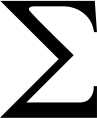
\includegraphics[width=0.225cm]{Bilder/Sigma.png} \nodepart{lower} 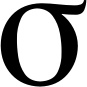
\includegraphics[width=0.225cm]{Bilder/sigma.png}};
        }
        % Draw the left input layer nodes
            \foreach \name / \xn in {1,...,\ni}{
            % This is the same as writing \foreach \name / \y in {1/1,2/2,3/3,4/4}
                \node[neuron,fontscale=15] (Il-\name) at (\xn*\neuronsep-\neuronsep,\y) {$i_{\xn}$};
                \node[above of=Il-\name, node distance=\inout cm] (Inl-\name) {};
                \draw [->,arrows={-Stealth[length=7pt]},densely dotted] (Inl-\name) edge (Il-\name);
            }
        % Draw the hidden layer node
            \foreach \name / \xn in {1,...,\nh}{
                \node[neuron,fontscale=15] (Hl-\xn) at ({(\ni-1)*\neuronsep/2-\neuronsep/2*(\nh-1)+(\xn-1)*\neuronsep},\y-\layersep) {$h_{\xn}$};
                \node[node distance=\inout cm, below of=Hl-\xn] (Hnl) {};
        % Connect every node in the inner layer with the hidden layer
            \foreach \source in {1,...,\ni}
                \draw [->,arrows={-Stealth[length=7pt]}] (Il-\source) edge (Hl-\xn);
                }
        % Draw the output layer node
            \foreach \name / \xn in {1,...,\no}{
                \node[neuron,fontscale=15] (Ol-\xn) at ({(\ni-1)*\neuronsep/2-\neuronsep/2*(\no-1)+(\xn-1)*\neuronsep},\y-2*\layersep) {$\Omega_{\xn}$};
                \node[node distance=\inout cm, below of=Ol-\xn] (Onl) {};
                \draw [->,arrows={-Stealth[length=7pt]},densely dotted] (Ol-\xn) edge (Onl);
        % Connect every node in the hidden layer with the output layer
            \foreach \source in {1,...,\nh}
                \draw [->,arrows={-Stealth[length=7pt]}] (Hl-\source) edge (Ol-\xn);
                }
        % Annotate the layers
            \ifthenelse{\ni>\nh}{
                \node[annot,right of=Il-\ni, node distance=\dlsize cm] (il) {\textbf{Eingabe- schicht}};
                \node[annot,below of=il] (hl) {\textbf{Verdeckte- schicht}};
            }{
                \node[annot,right of=Hl-\nh, node distance=\dlsize cm] (hl) {\textbf{Verdeckte- schicht}};
                \node[annot,above of=hl] (il) {\textbf{Eingabe- schicht}};
            }
                \node[annot,below of=hl] {\textbf{Ausgabe- schicht}};
        %-----------------------------------------
        %% rechtes Bild
            \tikzset{
                ident/.pic={
                \draw[semithick] (-\siz/4,-\siz/4) -- (\siz/4,\siz/4);
            }}
        % Draw the right input layer nodes
                \coordinate (tIr) at ($(il)-(Il-\ni)$);
                \coordinate (ttIr) at (tIr |- 0,0);
                \coordinate (Ir) at ($(il)+(ttIr)$);
            \foreach \name / \xn in {1,...,\ni}{
        % This is the same as writing \foreach \name / \y in {1/1,2/2,3/3,4/4}
                \node[neuron] (Ir-\name) at ($(Ir)+(\xn*\neuronsep-\neuronsep,0)$) {};
                \node[above of=Ir-\name, node distance=\inout cm] (Inr-\name) {};
                \pic at (Ir-\name) {ident};
                \draw [->,arrows={-Stealth[length=7pt]},densely dotted] (Inr-\name) edge (Ir-\name);
            }
        % Draw the right hidden layer node
            \foreach \name / \xn in {1,...,\nh}{
                \neurono[Hr-\xn]{$(Ir)+({(\ni-1)*\neuronsep/2-\neuronsep/2*(\nh-1)+(\xn-1)*\neuronsep},-\layersep)$}
                \node[node distance=\inout cm, below of=Hr-\xn] (Hnr) {};
        % Connect every node in the input layer with the hidden layer
            \foreach \source in {1,...,\ni}
                \draw [->,arrows={-Stealth[length=7pt]}] (Ir-\source) edge  (Hr-\xn);
            }            

                \node[fill=white,inner sep=1pt,fontscale=10] at ($(Hr-1)+({(\nh-1)*\neuronsep/2},\layersep*.5)$) {$\dots\,w_{i,h}\,\dots$};
        % Draw the right output layer node
            \foreach \name / \xn in {1,...,\no}{
                \neurono[Or-\xn]{$(Ir)+({(\ni-1)*\neuronsep/2-\neuronsep/2*(\no-1)+(\xn-1)*\neuronsep},-2*\layersep)$}
                \node[node distance=\inout cm, below of=Or-\xn] (Onr) {};
                \draw [->,arrows={-Stealth[length=7pt]},densely dotted] (Or-\xn) edge (Onr);
        % Connect every node in the hidden layer with the output layer
            \foreach \source in {1,...,\nh}
                \draw [->,arrows={-Stealth[length=7pt]}] (Hr-\source) edge  (Or-\xn);
            }
                \node[fill=white,inner sep=1pt,fontscale=10] at ($(Or-1)+({(\no-1)*\neuronsep/2},\layersep*.5)$) {$\dots\,w_{h,\Omega}\,\dots$};
\end{tikzpicture}
    \caption{MLP mit verdeckten Neuronen $h_n$ und einer verdeckten Schicht links bzw. zwei verdeckten Schichten rechts.}
    \label{fig:MLP}
\end{figure}

Im Unterschied zu den SLPs besitzen die Mehrschichtperceptrons zwischen der Eingabe- und Ausgabeschicht noch mindestens eine verdeckte Verarbeitungsschicht. Somit weisen sie mindestens zwei Ebenen an trainierbaren Gewichten auf. In \autoref{fig:MLP} sind MLPs mit einer und zwei verdeckten Schichten dargestellt. Die zusätzliche Ebene ermöglicht eine beliebig genaue Approximation einer Funktion mit endlich vielen Unstetigkeitsstellen und ihrer ersten Ableitung. Theoretisch können beliebig viele verdeckte Schichten aufgebaut werden aber wie \hbox{\citet{dkriesel07}} erläutert reichen drei Ebenen von trainierbaren Gewichten aus, um jede beliebige Menge darstellen zu können.\citef[86\,--\,89]{dkriesel07}

Um das MLP zu trainieren gibt es das sogenannt Backpropagation Verfahren das zu den überwachten Lernalgorithmen gezählt wird. Hierbei wird das Netzwerk in der Trainingsphase mit Informationen versorgt und das errechnete Ergebnis wird mit dem gewünschten Ergebnis verglichen. Die Abweichung wird anschließend genutzt, um die Gewichte ausgehend von den Ausgabe- hin zu den Eingabeneuronen anzupassen. Ein bekanntes Problem dieses Verfahrens ist dass bei mehreren Verdeckten Schichten und einer konstanten Lernrate, Gewichte langsamer trainiert werden je weiter sie sich von der Ausgabeschicht befinden.\citef[89\,--\,96]{dkriesel07} Des Weiteren hat eine hohe Anzahl an Ausgabeneuronen ebenfalls einen negativen Einfluss auf die Lerngeschwindigkeit des Netzwerkes.\citef[124]{dkriesel07}


\subsubsection{Radiale Basisfunktionen (RBF)}
\begin{figure}[!htb]
    \centering
    %---------------------------------------------------------------
        %% RBF
        %-----------------------------------------
        %% linkes Bild
        \begin{tikzpicture}[>=stealth', node distance=\layersep cm, shorten >=1pt]
        \def\layersep{1.8}          % vertikal distance between the layers
        \def\neuronsep{1.8}         % Horizontal distance between neurons
        \def\dlsize{2}              % distance between node and layer lable
        \def\inout{\layersep*.65}   % Size of in- and output-arrow
        \def\siz{.8}                % neuronsize
        \def\y{5}                   % Start of the most upper layer
        \def\ni{3}                  % Amount of input neurons
        \def\nh{4}                  % Amount of hidden neurons
        \def\no{2}                  % Amount of output neurons
        \tikzstyle{neuron}=[circle,draw=black,minimum size=\siz cm,inner sep=2pt]
        \tikzstyle{annot} = [text width=5em, text centered]
        \tikzset{fontscale/.style = {font={\fontsize{#1pt}{#1pt}\selectfont}}}
        \tikzset{
                ident/.pic={
                \draw[semithick] (-\siz/#1,-\siz/#1) -- (\siz/#1,\siz/#1);
            }}
        \newcommand{\neurono}[3][]{%
        \ifthenelse{\equal{#3}{0}}{%
            \node[neuron,circle split,inner sep=1pt,fontscale=6] (#1) at (#2)
                    { $\mathbf{||c,x||}$ \nodepart{lower} };
                    
            \node[fontscale=6] at ($(#2.lower)-(0,\siz/4)$){\textbf{Gauß}};
            }{
            \node[neuron,circle split,inner sep=1.3pt] (#1) at (#2)
                    {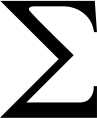
\includegraphics[width=0.225cm]{Bilder/Sigma.png} \nodepart{lower} };
            \pic at ($(#1.lower)-(0,\siz/8)$) {ident=#3};
            }}
        % Draw the left input layer nodes
            \foreach \name / \xn in {1,...,\ni}{
            % This is the same as writing \foreach \name / \y in {1/1,2/2,3/3,4/4}
                \node[neuron,fontscale=15] (Il-\name) at (\xn*\neuronsep-\neuronsep,\y) {$i_{\xn}$};
                \node[above of=Il-\name, node distance=\inout cm] (Inl-\name) {};
                \draw [->,arrows={-Stealth[length=7pt]},densely dotted] (Inl-\name) edge (Il-\name);
            }
        % Draw the hidden layer node
            \foreach \name / \xn in {1,...,\nh}{
                \node[neuron] (Hl-\xn) at ({(\ni-1)*\neuronsep/2-\neuronsep/2*(\nh-1)+(\xn-1)*\neuronsep},\y-\layersep) [fontscale=15] {$h_{\xn}$};
                \node[node distance=\inout cm, below of=Hl-\xn] (Hnl) {};
        % Connect every node in the inner layer with the hidden layer
            \foreach \source in {1,...,\ni}
                \draw [->,arrows={-Stealth[length=7pt]}] (Il-\source) edge (Hl-\xn);}
        % Draw the output layer node
            \foreach \name / \xn in {1,...,\no}{
                \node[neuron] (Ol-\xn) at ({(\ni-1)*\neuronsep/2-\neuronsep/2*(\no-1)+(\xn-1)*\neuronsep},\y-2*\layersep) [fontscale=15] {$\Omega_{\xn}$};
                \node[node distance=\inout cm, below of=Ol-\xn] (Onl) {};
                \draw [->,arrows={-Stealth[length=7pt]},densely dotted] (Ol-\xn) edge (Onl);
        % Connect every node in the hidden layer with the output layer
            \foreach \source in {1,...,\nh}
                \draw [->,arrows={-Stealth[length=7pt]}] (Hl-\source) edge (Ol-\xn);}
        % Annotate the layers
            \ifthenelse{\ni>\nh}{
                \node[annot,right of=Il-\ni, node distance=\dlsize cm] (il) {\textbf{Eingabe- schicht}};
                \node[annot,below of=il] (hl) {\textbf{Verdeckte- schicht}};
            }{
                \node[annot,right of=Hl-\nh, node distance=\dlsize cm] (hl) {\textbf{Verdeckte-/RBF- schicht}};
                \node[annot,above of=hl] (il) {\textbf{Eingabe- schicht}};
            }
                \node[annot,below of=hl] {\textbf{Ausgabe- schicht}};
        %-----------------------------------------
        %% rechtes Bild
        % Draw the right input layer nodes
                \coordinate (tIr) at ($(il)-(Il-\ni)$);
                \coordinate (ttIr) at (tIr |- 0,0);
                \coordinate (Ir) at ($(il)+(ttIr)$);
            \foreach \name / \xn in {1,...,\ni}{
        % This is the same as writing \foreach \name / \y in {1/1,2/2,3/3,4/4}
                \node[neuron] (Ir-\name) at ($(Ir)+(\xn*\neuronsep-\neuronsep,0)$) {};
                \node[above of=Ir-\name, node distance=\inout cm] (Inr-\name) {};
                \pic at (Ir-\name) {ident=4};
                \draw [->,arrows={-Stealth[length=7pt]},densely dotted] (Inr-\name) edge (Ir-\name);}
        % Draw the right hidden layer node
            \foreach \name / \xn in {1,...,\nh}{
                \neurono[Hr-\xn]{$(Ir)+({(\ni-1)*\neuronsep/2-\neuronsep/2*(\nh-1)+(\xn-1)*\neuronsep},-\layersep)$}{0}
                \node[node distance=\inout cm, below of=Hr-\xn] (Hnr) {};
        % Connect every node in the input layer with the hidden layer
            \foreach \source in {1,...,\ni}
                \draw [->,arrows={-Stealth[length=7pt]}] (Ir-\source) edge  (Hr-\xn);}
        % Draw the right output layer node
            \foreach \name / \xn in {1,...,\no}{
                \neurono[Or-\xn]{$(Ir)+({(\ni-1)*\neuronsep/2-\neuronsep/2*(\no-1)+(\xn-1)*\neuronsep},-2*\layersep)$}{6}
                \node[node distance=\inout cm, below of=Or-\xn] (Onr) {};
                \draw [->,arrows={-Stealth[length=7pt]},densely dotted] (Or-\xn) edge (Onr);
        % Connect every node in the hidden layer with the output layer
            \foreach \source in {1,...,\nh}
                \draw [->,arrows={-Stealth[length=7pt]}] (Hr-\source) edge  (Or-\xn);
            }
                \node[fill=white,inner sep=1pt,fontscale=10] at ($(Or-1)+({(\no-1)*\neuronsep/2},\layersep*.5)$) {$\dots\, w_{h,\Omega}\,\dots$};
        \end{tikzpicture}
    \caption{MLP mit verdeckten Neuronen $h_n$ und einer verdeckten Schicht links bzw. zwei verdeckten Schichten rechts.}
    \label{fig:RBF}
\end{figure}

RBFs sind feed-forward Netze und ähnlich wie die Perceptrons schichtartig aufgebaut. Dabei besitzt jedes Neuron einer Schicht eine Verbindung zu jedem Neuron der nachfolgenden Schicht (diese Art der Verbindung zwischen den Schichten wird auch Vollverknüpfung genannt). RBFs besitzen aber genau drei Schichten und somit nur eine verdeckte Schicht. Die erste Schicht dient ebenfalls wie bei den Perceptrons nur der Verteilung der Eingabedaten an die nächste Schicht ohne jegliche Verarbeitung. Die zweite Schicht besteht aus verdeckten Neuronen die auch als RBF-Neuronen bezeichnet werden. Jedes Neuron beinhaltet eine radiale Basisfunktion. Dies sind stets positive und radialsymmetrische Funktionen. Sie besitzen ein Maximum in der Mitte und streben gegen Null je weiter sich die Funktion vom Mittelpunkt entfernt. Eine typische Basisfunktion ist hierbei die gaußsche Glockenkurve. Die Ausgabe eines RBF-Neurons gibt daher Auskunft über die nähe der Eingabedaten zum Mittelpunkt der Basisfunktion. Schließlich sind die verdeckten Neuronen über eine gewichtete Verbindung mit den Ausgabeneuronen verknüpft. Die Ausgabeneurone summieren die Ausgabe der RBF-Neuronen und geben die Summe ohne weitere Verarbeitung weiter.

Ursprünglich wurden die RBFs als Interpolationsverfahren entwickelt. Daher wurde jedem Trainingsbeispiel ein Basispunkt und somit ein RBF-Neuron zugewiesen. Bei großen Datensätzen ergibt sich eine große Anzahl an verdeckten Neuronen die einen hohen Speicherbedarf nach sich ziehen. Um mit einer geringeren Anzahl an verdeckten Neuronen auszukommen können auch die RBF-Netze trainiert werden. Das Training der RBF-Netze findet oftmals in mehreren Stufen statt. Im ersten Schritt werden die Zentren und Formparameter durch unüberwachte Lernmethoden bestimmt. Im nächsten Schritt werden die Gewichte beispielsweise mit der Delta-Regel angepasst.

Die RBFs bieten den Vorteil dass durch das Stauchen/Strecken und Verschieben der Basisfunktionen und das anschließende Aufsummieren jede mögliche Funktion approximiert werden kann. Weiterhin wirkt sich die Anzahl an Ausgabeneuronen nicht wesentlich auf die Berechnungskomplexität aus. Im Gegenzug führt eine hohe Anzahl an Trainingsbeispielen aber auch zu einer gleich hohen Anzahl an verdeckten Neuronen und somit zu einem erhöhten Speicher- und Rechenaufwand. Eine Verringerung der Anzahl der RBF-Neuronen und anschließendes Training sind zwar möglich bestehen aber aus mehreren Stufen und erhöhen einerseits die Algorithmuskomplexität und bieten andererseits mehr Raum für Ungenauigkeiten.\footnote{Vgl. \citet[73\,--\,81]{comp_int_07}, \citet[109\,--\,125]{dkriesel07} und \citet[261\,--\,271]{Kroll16}.}



\subsubsection{Self Organizing Feature Maps (SOM)}

Die SOMs wurden in den 1980ern von Teuvo Kohonen vorgestellt und werden daher in der Literatur auch als Kohonen Netzwerke bezeichnet. Die SOMs sind nah verwandt mit RBFs. Sie bestehen aber aus zwei anstatt drei Schichten. Die Eingabeschicht dient auch der Informationsweitergabe an die Ausgabeschicht und ist mit dieser vollverknüpft. Die größte Ähnlichkeit zwischen SOM- und RBF-Netzen besteht in der Aktivierungsfunktion die bei SOMs ebenfalls eine radiale Funktion darstellt. Im Unterschied zu den RBFs liegen die Gewichte aber zwischen Eingabe- und Ausgabeschicht. Bei den SOMs ist es nun von Interesse welches Ausgabeneuron aktiv ist und nicht wie bei Perceptrons oder RBFs was die Neuronen berechnen. Zusätzlich sind die Neuronen der Ausgabeschicht abhängig von der Anwendung untereinander verbunden. Durch die Art der Verbindung ergibt sich die Dimension der Ausgabe.\footnote{Vgl. \citet[102\,--\,104]{Kruse15} und \citet[153\,--\,156]{dkriesel07}.}\farbig{BILD}

Trainiert werden die SOMs unüberwacht wobei die Neuronen bei der Eingabe der Testdaten um die Aktivität konkurrieren. Nach dem Prinzip ``the winner takes all'' werden nur die Gewichte des Neurons trainiert dessen Zentrum am kürzesten von dem Eingabewert liegt.\citef[272\,--\,275]{Kroll16}

So können SOMs hochdimensionale Daten auf eine niedrigdimensionale Karte abbilden, wobei die Nachbarschaftsbeziehung der Daten erhalten bleibt.\citef[7]{Kramer09} Dies ermöglicht qualitativ die Nachbarschaftsbeziehungen zu visualisieren und Zusammenhänge von Daten durch Anhäufungen von Neuronen zu finden. Hieraus folgt dass SOMs bei der Vorselektion von Daten eingesetzt werden können sind aber für die Approximation von Funktionen weniger geeignet.

\subsection{Gegenüberstellung der Netzwerke}


%\subsubsection{Fuzzy-neuronales Netz}

%\newpage
%\lipsum

%\subsubsection{Hopfield Netzwerk}

%\subsection{Multilayerperceptrons (MLP)}

%\subsection{Radiale Basisfunktionen (RBF)}

%\subsection{Gegenüberstellung von MLP- und RBF-Netzen}